\section{扩展}
\label{kvdirect:sec:extensions}

\subsection{基于 CPU 的分散 - 聚集 DMA}


对于64B DMA操作,PCIe具有29%的TLP报头和填充开销(\S \ref {kvdirect:sec:challenge}),并且DMA引擎可能没有足够的并行性来使用小TLP使PCIe带宽延迟积(BDP)饱和。
系统中的PCIe根(root complex)支持更大的DMA操作,最高256字节的TLP有效负载。 在这种情况下,TLP头和填充开销仅为9%,并且DMA引擎具有足够的并行性(64)以通过27个正在进行的DMA读取来使PCIe链路饱和。
要批量处理PCIe链路上的DMA操作,可以利用CPU来执行分散 - 聚集(scatter gather)(图 \ref {kvdirect:fig:sg-arch})。
首先,网卡 DMA将地址发送到主机内存中的请求队列。主机CPU轮询请求队列,执行随机内存访问,将数据放入响应队列并将MMIO门铃写入网卡。然后,网卡通过DMA从响应队列中提取数据。


\begin{figure}[htbp]
		\centering
		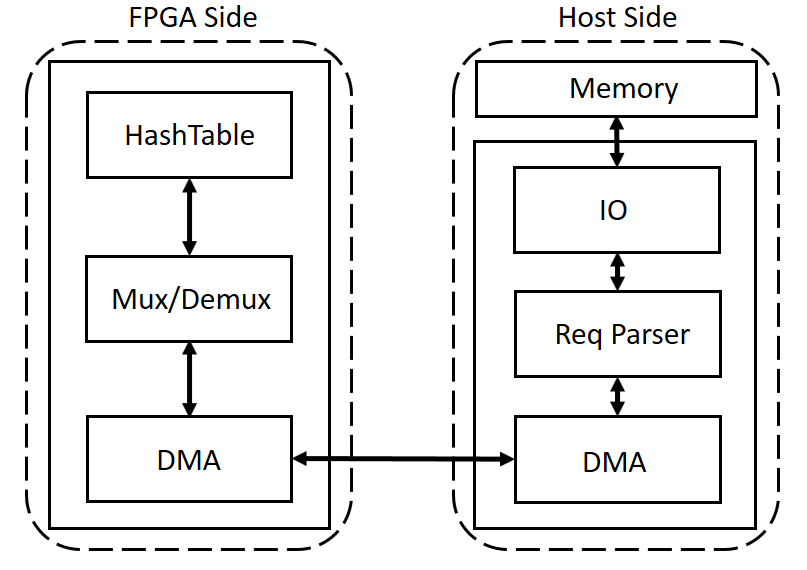
\includegraphics[width=0.6\textwidth,page=1]{scatter_gather.PNG}
		\caption{分散 - 聚集(scatter-gather)架构。}
		\label{kvdirect:fig:sg-arch}
\end{figure}


图 \ref {kvdirect:fig:scatter-gather} 表明,与CPU旁路方法相比,基于CPU的分散 - 聚集DMA的吞吐量提高了79%。
除了CPU开销之外,基于CPU的分散 - 聚集的主要缺点是额外的延迟。
为了将MMIO从CPU保存到网卡,每个门铃批量256个DMA操作,这需要 10 $\mu$s 才能完成。
使用基于CPU的分散 - 聚集网卡访问主机内存的总延迟是大约20美元,比直接DMA高出近20倍。




\begin{figure}[htbp]
	\centering
	\subfloat[读操作。\label{kvdirect:fig:sge-read}]
	{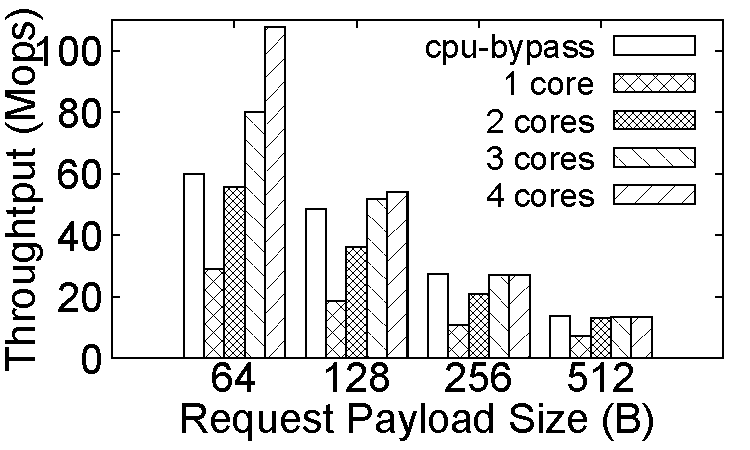
\includegraphics[width=.5\textwidth,page=1]{sg-read.pdf}}
	\subfloat[写操作。\label{kvdirect:fig:sge-write}]
	{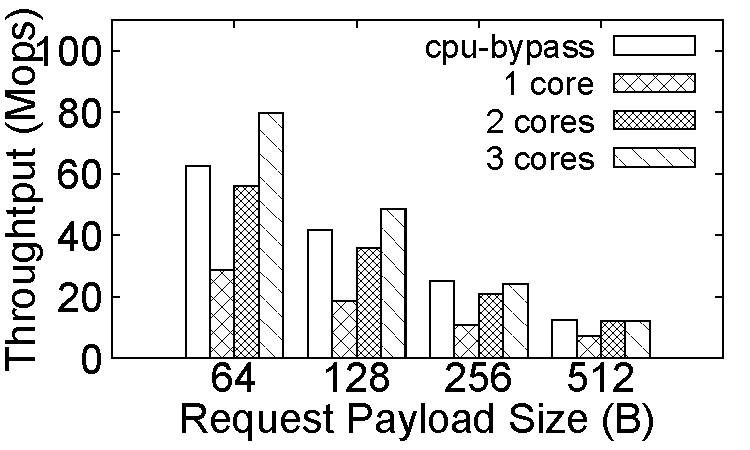
\includegraphics[width=.5\textwidth,page=1]{sg-write.pdf}}
	\caption{分散 - 聚集(scatter-gather)性能。}
	\label{kvdirect:fig:scatter-gather}
\end{figure}


\subsection{单机多网卡}
\label{kvdirect:sec:multi-nic}

KV-Direct的主要用例是启用远程直接键值访问,而无需服务器上的CPU开销。
在某些情况下,可能需要构建一个具有每服务器最大吞吐量的专用键值存储。
通过模拟,\cite {li2016full}显示了在具有四个(当前不可用的)60核CPU的单个服务器中实现十亿键值运行的可能性。
如表 \ref{kvdirect:tab:kvs-compare} 所示,在服务器上有10个KV-Direct 网卡,使用商用服务器可以轻松实现10亿键值 op/s性能。

如图 \ref{kvdirect:fig:photo},服务器消耗357瓦的功率(在墙壁上测量)以达到1.22~Gop/s GET或0.61~Gop/s PUT 的性能。


\begin{figure}[htbp]
	\centering
	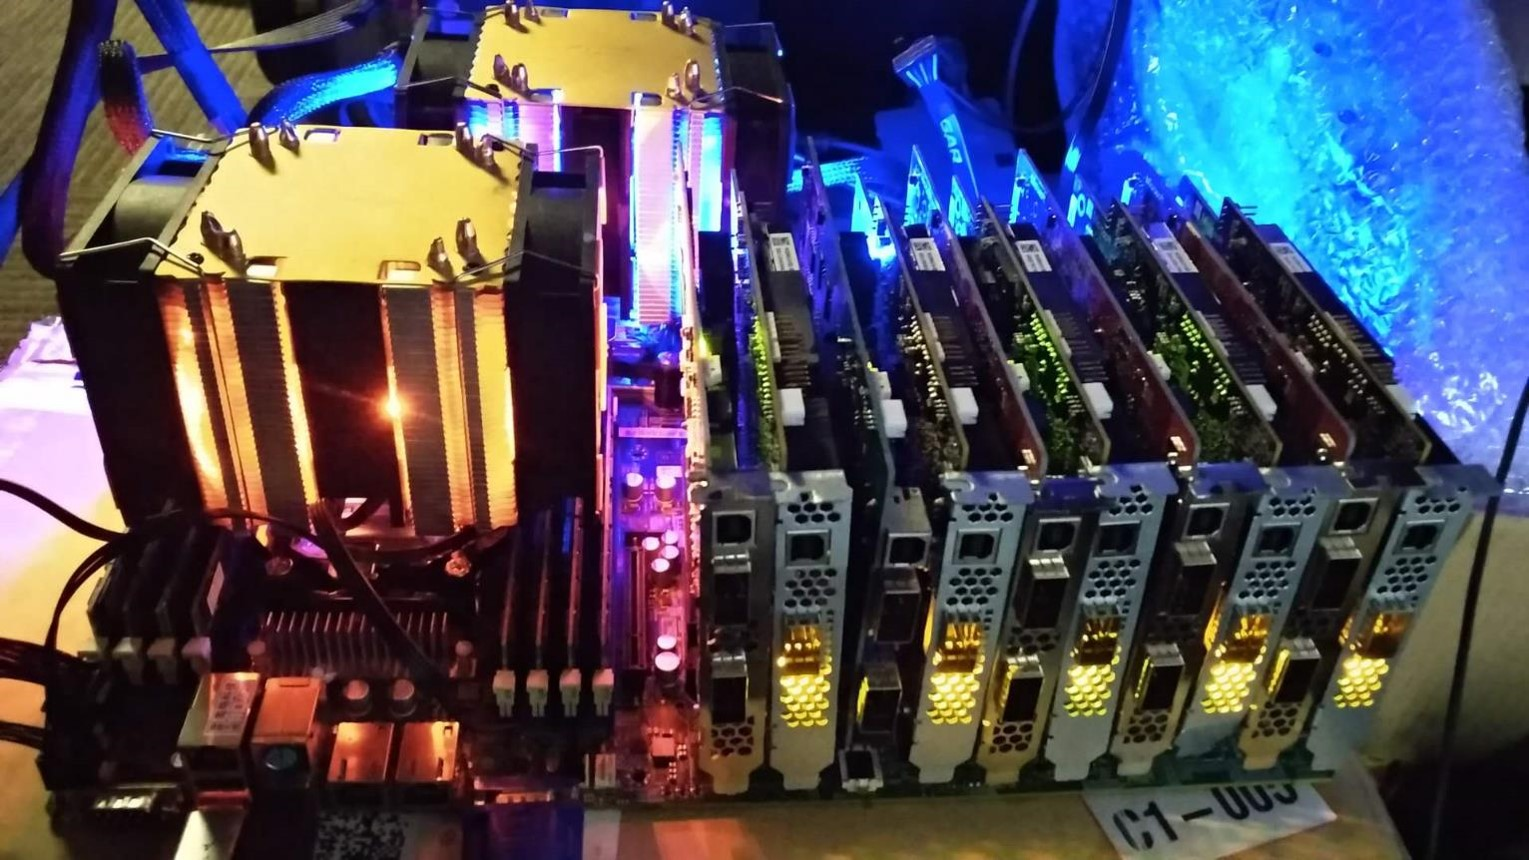
\includegraphics[width=0.9\textwidth]{figure/kvdirect_photo.jpg}
	\caption{以 357 瓦功耗实现 12.2 亿次键值操作每秒的 10 卡 KV-Direct 系统。}
	\label{kvdirect:fig:photo}
\end{figure}

为了使两个Xeon E5 CPU的80个PCIe Gen3通道饱和,用带有10个PCIe Gen3 x8插槽的 SuperMicro X9DRX+-F 主板替换了基准测试服务器的主板,PCIe 拓扑如图 \ref{kvdirect:fig:pcie_topology} 所示。


\begin{figure}[htbp]
	\centering
	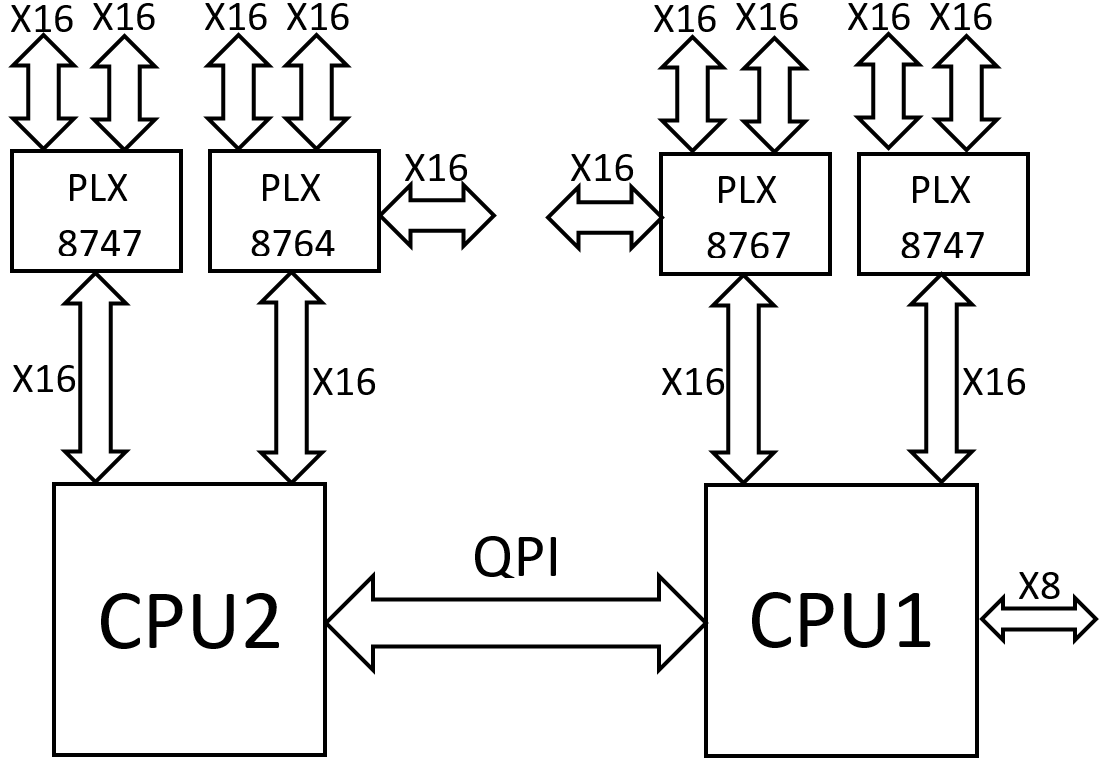
\includegraphics[width=0.5\textwidth]{figure/pcie_topology.PNG}
	\caption{10 卡 KV-Direct 系统的 PCIe 拓扑图。}
	\label{kvdirect:fig:pcie_topology}
\end{figure}


使用PCIe x16到x8转换器连接每个插槽上的10个可编程网卡,每个网卡上只启用一个PCIe Gen3 x8链路,因此每个网卡的吞吐量低于图 \ref {kvdirect:fig:ycsb-tput}。
每个网卡在主机内存中拥有一个独占内存区域,并提供不相交的键分区。
多个网卡遇到与多核键值存储实现相同的负载不平衡问题。
幸运的是,对于少量分区(例如10个),负载不平衡并不重要 \cite {lim2014mica,li2016full}。在YCSB长尾工作负载下,负载最高的网卡的平均负载为1.5倍,非常流行的键所增加的负载由无序执行引擎提供(\S \ref {kvdirect:sec:ooo})。
相比之下,为了实现与240个CPU内核的匹配性能,最热 CPU 核心的负载将是平均值的10倍。
图\ref {kvdirect:fig:multiple-nics}显示KV-Direct吞吐量几乎与服务器上的网卡数量呈线性关系。


\begin{figure}[htbp]
	\centering
	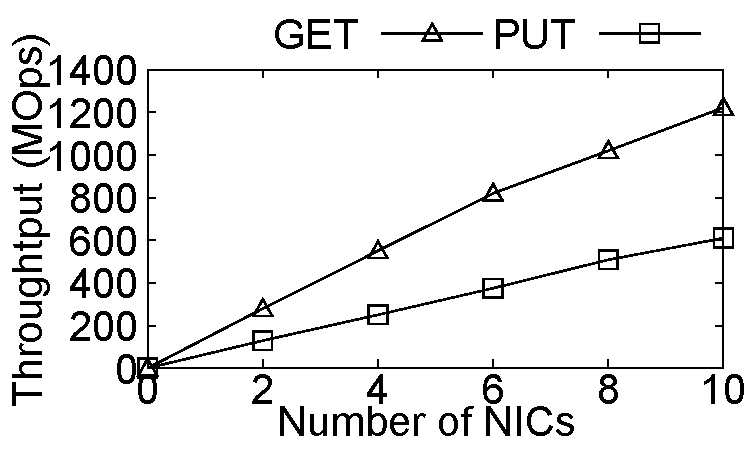
\includegraphics[width=0.5\textwidth,page=1]{multi_nic.pdf}
	\caption{单机多网卡的性能可扩放性。}
	\label{kvdirect:fig:multiple-nics}
\end{figure}


\subsection{基于 SSD 的持久化存储}

基于内存数据结构存储断电后数据会丢失。为了持久化,本节利用 SATA SSD 实现了持久化键值存储。由于服务器上的 SSD 数量是有限的,且操作系统和应用程序也运行在 SSD 上,键值存储需要与操作系统和应用程序共享 SSD 硬件。
为此,SSD 提供块存储(block storage)和键值存储两种访问接口。与内存键值存储采用专门预留的内存空间类似,键值存储也位于专门预留的块存储空间内。
CPU 需要两种访问块存储的方式:一是通过操作系统的存储协议栈来访问块设备,二是通过用户态的快速接口绕过操作系统直接访问。
由于操作系统本身和很多软件运行在块存储上,保持第一种传统访问方式的兼容性是必要的。
存储性能敏感的应用则使用本文提供的运行库来通过第二种方式访问块存储。


\begin{figure}[htbp]
	\centering
	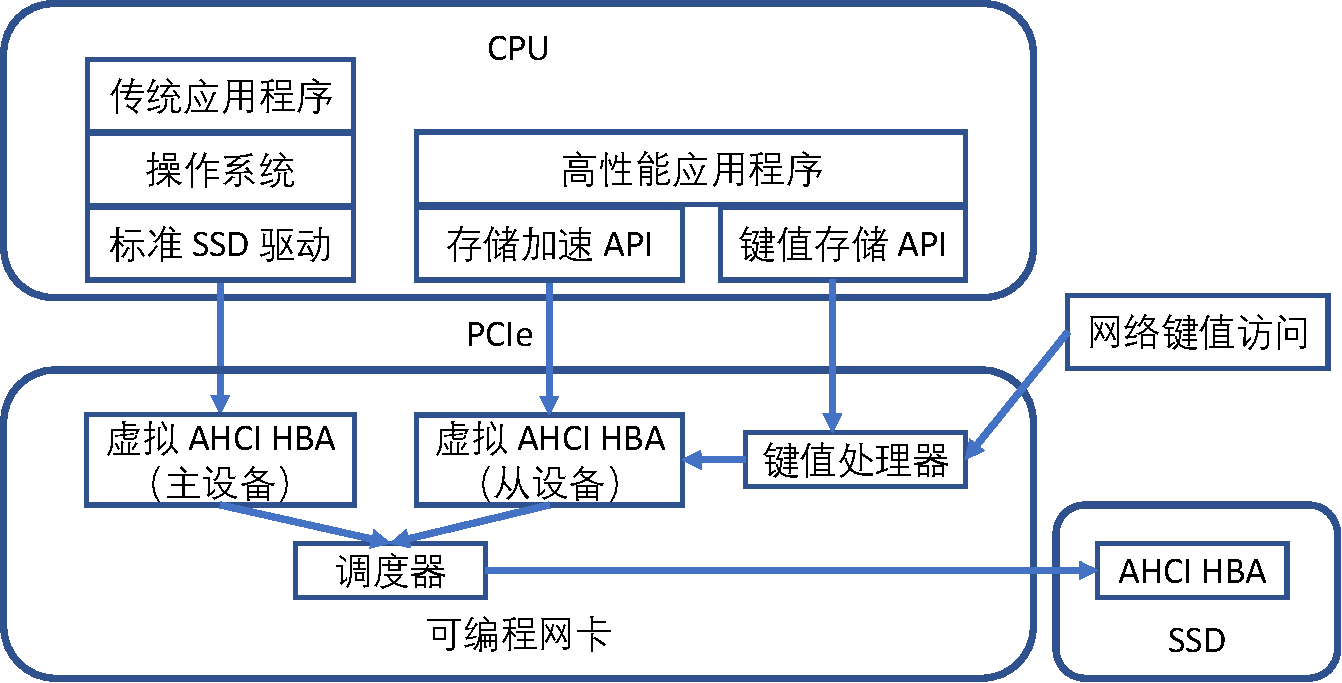
\includegraphics[width=0.9\textwidth]{ssd.pdf}
	\caption{SSD 持久化存储架构。}
	\label{kvdirect:fig:ssd}
\end{figure}

如图 \ref{kvdirect:fig:ssd},可编程网卡将 SSD 虚拟化成两个虚拟 AHCI HBA 设备。
可编程网卡内的调度器将存储硬件的数据平面(如 SATA 的 32 个请求槽位和 NVMe 的请求队列)虚拟化成两个逻辑存储设备。
存储硬件的控制寄存器(如 PCIe 配置寄存器)透传给主逻辑存储设备,由原有的操作系统管理。
从逻辑存储设备没有控制面,仅有数据面,只能进行数据读写,不能进行管理操作。
上述存储虚拟化架构无需可编程网卡管理控制面,简化了调度器的设计;而且保持了与原有存储设备驱动程序和操作系统的兼容性。
如图 \ref{kvdirect:fig:ssd-benchmark},存储虚拟化后通过主逻辑存储设备和原有的操作系统和软件的顺序访问吞吐量没有明显变化。延迟从约 30 $\mu$s 升高到了约 60 $\mu$s,这是可编程网卡转发的开销。由于延迟增加,单线程随机访问(4K 块大小)的吞吐量也有所降低。在 64 个线程随机访问时,由于 SATA 只有 32 个请求槽位,即只能并行进行 32 个读写请求,吞吐量受限于请求的平均延迟。

\begin{figure}[htbp]
	\centering
	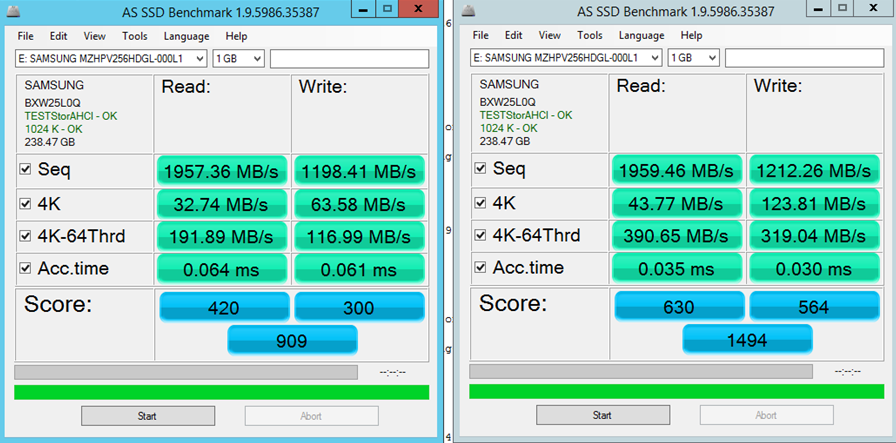
\includegraphics[width=0.8\textwidth]{storahci.png}
	\caption{SSD 虚拟化的性能评估。左图为存储虚拟化后原有操作系统和 SSD 性能测试程序的结果。右图为不使用存储虚拟化时该 SSD 的性能测试结果。}
	\label{kvdirect:fig:ssd-benchmark}
\end{figure}

为了提供高效的块设备访问接口,本节利用第 \ref{chapter:clicknp} 章的 PCIe I/O 管道,使应用程序可以通过存储加速 API 直接访问可编程网卡,绕过操作系统和驱动程序。
存储加速 API 可以访问 SSD 上任意的存储块,避免与操作系统的文件系统冲突是应用程序的责任。通常,应用程序创建一个大文件以预留存储空间。
实验表明,仅用单个 CPU 线程,存储加速 API 就可以充分利用 SSD 约 2 GB/s 的顺序读写吞吐量和约 50 K 次每秒的 4K 块大小随机读写吞吐量。
传统操作系统存储协议栈需要 8 个 CPU 线程才能充分利用 4K 块大小随机读写的吞吐量。
为了提供持久化的键值存储,键值处理器连接到虚拟存储的从设备上,把虚拟存储当作一大块内存来读写。
本文没有针对 SSD 的读写特性进行优化,这将是未来的工作。






\subsection{分布式键值存储}

在分布式键值存储中,我们假设每台主机既是使用键值存储的客户端,又能分配一些内存资源作为键值服务器。
每个键值对需要在多个服务器节点上复制,以提供高可用性,并提高键值访问的性能。
传统的键值存储服务简单地根据键的哈希值选定服务器。然而,并不是每台主机都以相同的概率访问每个键。例如,图计算中一台主机如果负责处理一个顶点,那么访问该顶点对应的键值的概率将高于其他主机。这时,该顶点的键值对最好存储在该主机上,以便利用局部性加速访问。

分布式存储系统需要决定每个键值对在哪些主机上复制。读操作只需读取最近的副本。写操作则需要通过主节点(master)同步到所有的副本。如果复制份数过多,主节点将写操作同步到各个副本会成为瓶颈。为了平衡主节点与各个副本节点的负载,复制的份数取决于读写比例。假定读写操作的比例为 $R$,且 $R$ 远大于 1 \footnote{在写入密集型负载中,如果仅有一个主节点,不做任何复制显然是性能最优的。为了高可用性,可能需要限制副本的最小数量。}。可以推导得出,当主节点与副本节点的负载相等时,复制的份数约为 $\sqrt{R}$。相比单个副本,读操作的负载降低了约 $\sqrt{R}$ 倍;相比复制到每个主机,写操作的负载降低了约 $\sqrt{R}$ 倍。

决定复制的份数后,下一个问题是选定读取最频繁的主机来复制。本文在主节点的可编程网卡内为每个键分别维护读次数、写次数的近似计数器 \footnote{近似计数器是为了节约存储空间。例如,近似计数用 11 位真数(significand)和 5 位幂数(exponent)的浮点数表示。每次访问时以 2 的幂数次方分之一的概率将真数加 1。}。在写操作同步到各个副本时,主节点汇总所有副本的读次数。根据读写次数之比可以计算出最佳副本数量,并在与当前副本数量相差较多时增加或减少副本数量,使得副本存储在读次数最多的若干节点上。为了防止写操作稀少导致主节点不能及时响应大量的读请求,副本节点在收到大量读请求后也可以主动向主节点汇报。

另一个问题是一些键的访问频率可能很高,以至于单机吞吐量可能成为瓶颈。例如,分布式事务中的序列号发生器、热门网络资源的访问计数器和共享资源的锁需要高吞吐量的单键原子操作。最近的 NetCache \cite{netcache-sosp17}、NetChain \cite{jin2018netchain} 等工作使用可编程交换机作为缓存,获得了比单个主机更高的单键读写性能,但仍然受到交换机性能的限制。

本文提出,使用多主复制(multi-master replication),单键读写性能可以随主机数量扩放,并保证强一致性。保证一致性的机制是令牌环(token ring),任意时刻有且仅有一个持有令牌的节点在处理写操作。令牌在各个主节点组成的环上按顺序传递,并附带当前最新的值。令牌环能够提升单键性能的关键是读写操作和很多原子操作是可结合(associative)的。例如,多个写操作可被归约为最后一次写操作;多个原子加减操作可以归约为一次原子加减操作;比较并交换的原子操作较为复杂,但多个操作也可以归约为一张大小不超过原子操作数量的查找表。因此,当一个节点不持有令牌时,就将收到的操作记录在缓冲区内,并归约这些操作。在令牌到来时,节点可以迅速在最新值的基础上执行归约后的操作,并将更新后的值随令牌发送给下一节点。此后,节点重放缓冲区内的操作并将每个操作的结果返回给客户端。
理论分析表明,在请求均匀到达各个主节点时,系统的吞吐量和平均延迟都随主节点数量线性增加。最坏延迟是令牌环转一圈所需的时间。由于缓冲区内的操作被归约,每个节点的处理延迟是有界的,令牌环转一圈的时间也就有界。每个主节点所需的请求缓冲区大小等于最坏延迟与网络带宽的乘积。
令牌环的开销是一个在网络中不断传递的数据包,即使没有读写请求,令牌也要在网络中不断传递。

实际的键值存储系统不只有一个访问频繁的键。为每个键设置一个令牌的网络开销过高,因此本文使用一个令牌服务所有的键。
然而,等待所有键都处理完成后再集中发送有更新的所有键值对,会带来较高的延迟。
假设一段时间内访问的键是随机的,也就是大多数键值操作涉及的键是不重复的。此时,令牌所附带的键值更新大小与缓冲区内的键值操作数量成正比,传输这些键值更新的时间不再是有界的,因此请求延迟会随负载因子接近 1 而趋于无穷大。
为此,本文将相邻的主节点间流水线化键值处理和传输。主节点将缓冲区内的键值操作组织成按照键递增排序的优先队列,键值更新也按键递增顺序发送,令牌标示键值更新序列的尾部。当主节点收到键 $K$ 的更新时,缓冲区内不超过 $K$ 的键值操作就可以被处理,并沿令牌环发送到下一主节点。这样,令牌环上的多个主节点可以并发处理不同的键,即令牌传递方向上靠前的主节点处理较小的键。理论分析表明,在请求的键服从均匀分布且请求均匀到达各个主节点时,请求延迟仍然是有界的,与负载因子无关,且仅比单键情形下的延迟略高。


\section{讨论}
\label{kvdirect:sec:discussion}

\subsection{不同容量的网卡硬件}
\label{kvdirect:sec:different-nic}

KV-Direct的目标是利用数据中心的现有硬件来卸载重要的工作负载(键值访问),而不是设计特殊的硬件来实现最大的键值存储性能。可编程网卡通常包含有限数量的DRAM用于缓冲和连接状态跟踪。 大型DRAM在芯片尺寸和功耗方面都很昂贵。

即使未来的网卡具有更快或更大的板载内存,在长尾工作负载下,本文的负载分配设计(\S \ref {kvdirect:sec:dram-cache})仍然显示出比简单的分区设计更高的性能。键统一根据网卡和主机内存容量。
表 \ref {kvdirect:tab:optimal-load-dispatch} 显示了具有10亿个键的长尾工作负载的最佳负载分配比率,不同的网卡 DRAM和PCIe吞吐率以及不同的网卡和主机比率内存大小。
如果网卡具有更快的DRAM,则将更多负载分派给网卡。负载分配比率为1表示网卡内存的行为与主机内存的高速缓存完全相同。
如果网卡具有更大的DRAM,则将稍微少量的负载分派给网卡。
如表 \ref {kvdirect:tab:optimal-load-dispatch-throughput} 所示,即使网卡 DRAM的大小只是主机内存的一小部分,吞吐量增益也很大。


\begin{table}[htbp]
	\centering
	\caption{不同网卡 DRAM / PCIe吞吐率(垂直)和网卡 /主机内存大小比(水平)下长尾工作负载的最佳负载分配比。}
	\label{kvdirect:tab:optimal-load-dispatch}
	\small
	\begin{tabular}{|l|r|r|r|r|r|r|}
		\hline
		& 1/1024 & 1/256 & 1/64 & 1/16 & 1/4 & 1 \\
		\hline
		1/2  & 0.366 & 0.358 & 0.350 & 0.342 & 0.335 & 0.327 \\
		\hline
		1    & 0.583 & 0.562 & 0.543 & 0.525 & 0.508 & 0.492 \\
		\hline
		2    & 0.830 & 0.789 & 0.752 & 0.718 & 0.687 & 0.658 \\
		\hline
		4    & 1     & 0.991 & 0.933 & 0.881 & 0.835 & 0.793 \\
		\hline
		8    & 1     & 1     & 1     & 0.995 & 0.937 & 0.885 \\
		\hline
	\end{tabular}
\end{table}


\begin{table}[htbp]
	\centering
	\caption{与简单分区相比,负载分派的相对吞吐量。行列标题与表 \ref{kvdirect:tab:optimal-load-dispatch} 相同。}
	\label{kvdirect:tab:optimal-load-dispatch-throughput}
	\small
	\begin{tabular}{|l|r|r|r|r|r|r|}
		\hline
		& 1/1024 & 1/256 & 1/64 & 1/16 & 1/4 & 1 \\
		\hline
		1/2 & 1.36	& 1.39	& 1.40	& 1.37	& 1.19	& 1.02 \\ 
		\hline
		1	& 1.71	& 1.77	& 1.81	& 1.79	& 1.57	& 1.01 \\
		\hline
		2	& 2.40	& 2.52	& 2.62	& 2.62	& 2.33	& 1.52 \\
		\hline
		4	& 3.99	& 4.02	& 4.22	& 4.27	& 3.83	& 2.52 \\
		\hline
		8	& 7.99	& 7.97	& 7.87	& 7.56	& 6.83	& 4.52 \\
		\hline
	\end{tabular}
\end{table}


乱序执行引擎(\S \ref {kvdirect:sec:ooo})可以应用于需要隐藏延迟的各种应用程序,本文希望未来的RDMA 网卡能够支持更更性能的原子操作。

在40~Gbps网络中,网络带宽限制了非批量键值吞吐量,因此本文使用客户端批处理。通过更高的网络带宽,可以减少批量大小,从而减少延迟。在200~Gbps网络中,KV-Direct网卡无需批量即可达到180~Mop/s。

KV-Direct利用广泛部署的可编程网卡和FPGA实现 \cite{putnam2014reconfigurable,caulfield2016cloud}。 FlexNIC \cite {kaufmann2015flexnic,kaufmann2016krishnamurthy} 是另一种具有可重构匹配行动表(RMT) \cite {bosshart2013forwarding} 的可编程网卡的有前途的架构。
NetCache \cite {netcache-sosp17} 在基于RMT的可编程交换机中实现键值缓存,显示了在基于RMT的网卡中构建KV-Direct的潜力。

\subsection{对现实世界应用的影响}

当KV-Direct应用于端到端应用程序时,后台计算显示了潜在的性能提升。 在PageRank \cite {page1999pagerank}中,由于每次边缘遍历都可以通过一次键值操作实现,因此KV-Direct在具有10个可编程网卡的服务器上支持1.22G TEPS。 相比之下,GRAM \cite {wu2015g}支持每台服务器250M TEPS,受交错计算和随机内存访问的约束。

KV-Direct支持用户定义的函数和向量操作(表 \ref {kvdirect:tab:kv-operations}),可以通过将客户端计算卸载到硬件来进一步优化PageRank。 类似的参数适用于参数服务器 \cite {li2014scaling}。本文希望未来的工作可以利用硬件加速的键值存储来提高分布式应用程序的性能。

\subsection{可编程网卡内的有状态处理}

本文第 \ref{chapter:clicknp} 章的 ClickNP 架构比较适合无状态或状态简单的流水线式数据包处理,而对基于连接状态或应用层请求的处理,就显得捉襟见肘。
例如,四层负载均衡器应用中的调度器和哈希表与应用逻辑耦合紧密,既不容易扩放到大量并发连接,代码的可维护性也不强。事实上在开发过程中花费了大量的时间来解决死锁问题。
为此,本章提出的有状态处理(stateful processing)和哈希表数据结构设计等基础组件可以作为很多可编程网卡应用的基础,如第 \ref{chapter:clicknp} 章的有状态网络功能(如四层负载均衡器)和第 \ref{chapter:socksdirect} 章的可扩放 RDMA。


\begin{figure}[htbp]
	\centering
	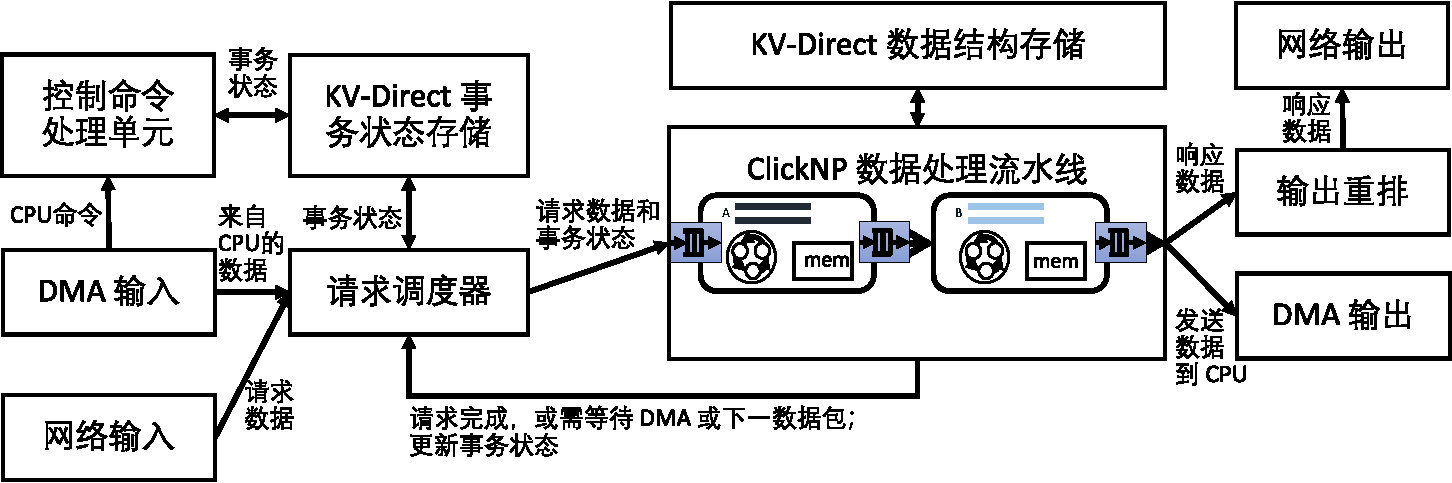
\includegraphics[width=1.0\textwidth]{../figures/kvdirect_arch.pdf}
	\caption{基于 KV-Direct 的可编程网卡应用层架构。}
	\label{arch:fig:kvdirect_arch}
\end{figure}


为了模块化和可扩放性,使用 KV-Direct 作为基础后,可编程网卡上应用的架构如图 \ref{arch:fig:kvdirect_arch} 所示。
事务代表着前后依赖关系,例如有状态网络处理中的一个连接,分多个数据包的一个应用层 HTTP 请求,或者键值存储中对同一个键(key)的操作。
同一个事务中的不同请求需要依次处理,而不同事务中的请求可以并发处理。
为了隐藏延迟、最大化并发处理能力,请求调度器从基于 KV-Direct 的事务状态键值存储中查找该请求对应的事务编号,并将正在处理事务的请求排入队列。
基于 ClickNP 的数据处理流水线根据请求数据和事务状态进行处理,在处理过程中可能查询其他的数据结构(如内存分配表、主机虚拟地址映射表、防火墙规则表、路由表等)。
如果请求处理完成,响应数据进入输出重排模块,重新排列响应的顺序以满足事务处理的一致性要求(例如,不同事务的请求也要按照到达顺序依次响应),最终输出到网络。
如果请求的处理还需要依赖下一数据包或从主机内存 DMA 来的数据,为了不阻塞数据处理流水线,该请求会返回到调度器,等待依赖操作完成后再进行下一阶段的处理。

